% !TeX spellcheck = en_GB

	In this chapter we are going to explain the different resources we have chosen to create an approach that allowed us to implement our final models. First, we include a detailed description of the database that we have chosen in section \ref{section:audioset}. Then, we comment and analyze the system we are going to employ so as to obtain high level features for our classification experiments in section \ref{section:feature-extractor}. In this point, the model is itemized step by step and also a theoretical explanation is included in \ref{subsection:ann-cnn}.
	
\section{Database: AudioSet}
\label{section:audioset}

\subsection{What is AudioSet} \todo{How cite? CPM: como misc, por ejemplo en la página web y con el artículo que la describe}
\label{subsection:what-is-audioset}

	Audio Set can be described as a large-scale sound dataset with the goal of putting the availability of audio and image data on the same level. It is composed by a huge variety of 2,084,320 manually-annotated audio events in video format and it is organized by following an ontology formed by 632 different audio classes. The data has been extracted from YouTube videos and the labelling process has been based on diverse factors such as metadata, context and content analysis. It has been developed by Google with the purpose of producing an audio event recognizer that can be applied to plenty of acoustic situations coming from the real world \cite{Gemmeke2017}.
	
	Due to some limitations found during the building process that will be explained along the section, the current final release of the dataset is composed by 1,789,621 segments, where each video usually last 10 seconds which results in a total duration of 4,971 hours of video and audio. After executing the selection process in which the different labels were populated with the final corresponding segments, a total of 527 classes were gathered, out of which 485 counted with at least 100 samples.

\subsection{Ontology}
\label{subsecition:ontology}

	In order to put this dataset together the events have been organized in an abstract hierarchy. This is composed by higher-level classes which describe a certain type of sound event and also act as parents of other labels that refer to more specific events. With this purpose, the relationship among different classes needs to be non-exclusive, so labelling similar audio events may result into a more general class, the parent, if there was ambiguity. This is also helpful for labellers due to group the clips in an easier and faster way.
	
	The Audio Set Ontology was collected considering some fundamental guidelines explained below:
	% List
	% !TeX spellcheck = en_GB
\begin{itemize}
	\item \doubt{A complete collection of all labels must be prepared} so that it can be used to define sound events from real-world aural data.
	\item When labelling an audio event the result must match the criteria of a common listener.
	\item Different categories should be easy to distinguish by an ordinary listener. In the case that two different labels do not satisfy this requirement, these should be merged. With this condition, the spectrum of possible labels remains limited.
	\item The distinction of two different classes must be done by relying just on the audio, it cannot be accompanied by image or visual information.
	\item The hierarchy should not be very deep by keeping the number of children per parent class to no more than 10. This also eases the annotation labour. 
\end{itemize}

	
	It is easy that an ontology of this volume gets leaned or biased towards a particular direction due to several factors, such as the subjectiveness of its creators or the selection of the initial set of classes used when starting to label. With the intention of generating a primary list that covers a wide range of audio events in an objective way, the researchers decided to apply an impartial, web-scale text analysis from the very beginning. They agreed on detecting hyponyms of the word "sound" by utilizing a modified version of the famous technique called \textit{Hearst patterns} \cite{Hearst1992}, a method proposed to automatically acquire hyponymy lexical relations from unrestricted text. As a result, an enormous collection of terms came up. This was filtered by considering how well these terms represented audio, i.e. by combining together the global frequency of occurrence and how exclusively these are recognized as hyponyms of "sound" instead of other terms. As an output of the final process, a list of 3000 terms was obtained.
	
	With respect to the hierarchical relation among categories, it was constructed by the authors with the main intention that this satisfied their human comprehension of the sounds. Event though this is a subjective manner, it also makes sense since this is how the hierarchy best performs its labour on helping human labelling.
	After all the organization process, the model is not based on a strict organization as a singular node can appear in many different locations, i.e., a single node can be child of different parent nodes. As we said before, the final result is composed by 632 audio event labels and, in the hierarchy, the deepest class is six level away from the top parent. Figure \ref{fig:mesh1} shows the nodes that belong to the two top layers of the ontology.
	
	% Figure of ontology
	\begin{figure}[h]
		\centering
		\captionsetup{justification=centering}
		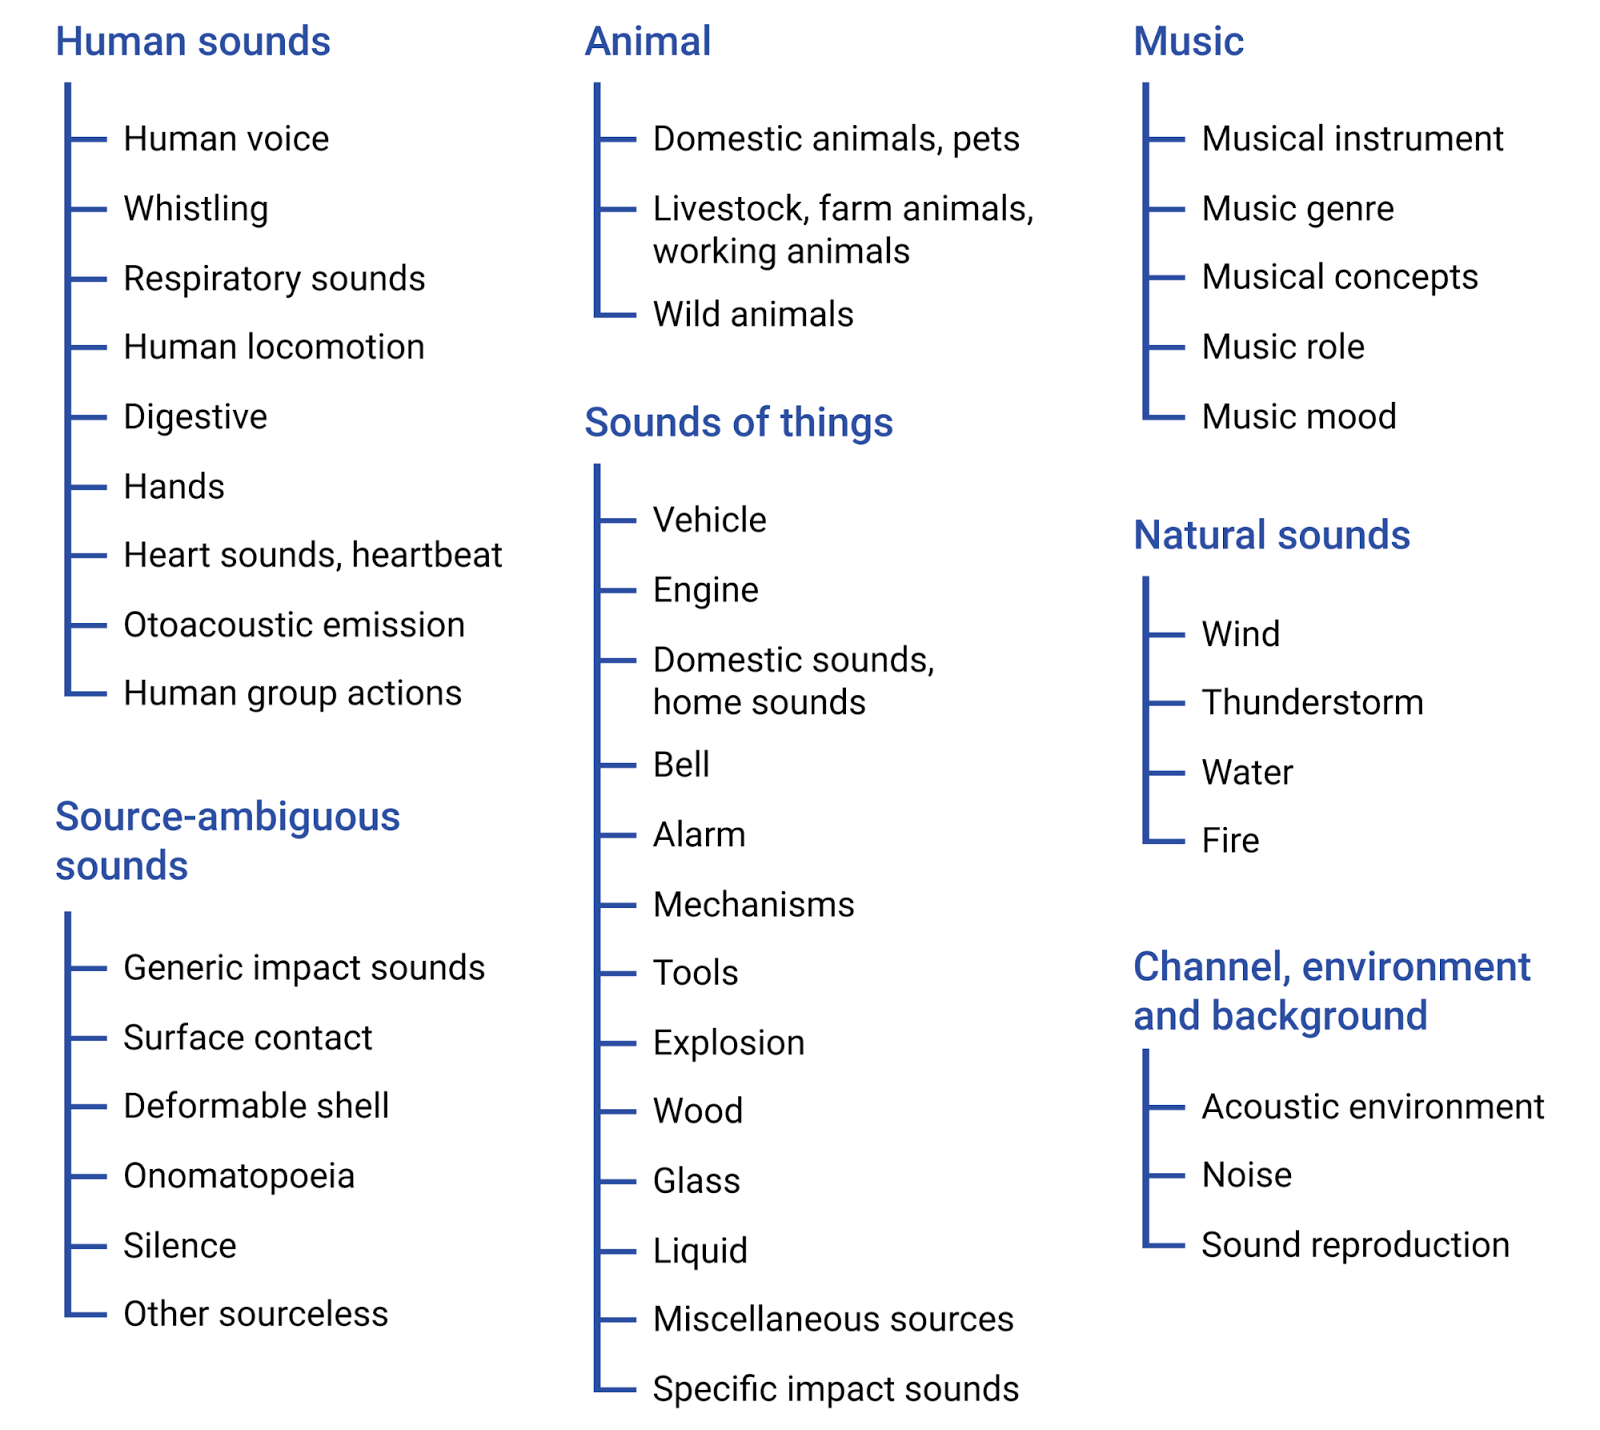
\includegraphics[scale=0.21]{audioset-ontology}
		\caption{First two layers of Audio Set Ontology \cite{Gemmeke2017}}
		\label{fig:mesh1}
	\end{figure}
	
	This whole structure is offered to any user as a file in JSON format. A couple of fields have been included for each label in order to describe its meaning and make clear its position within the hierarchy. A description for all of these can be found in table \ref{table:2}. 
	
	% !TeX spellcheck = en_GB
% Ontology-fields table

\begin{table}[h!]
\begin{center}
	\begin{tabular}{|| m{7em} | m{22em} ||}
		\hline
		ID & This field includes the Knowledge Graph \acrfull{mid} that best describes the sound or its source. It is used as a primary identifier for the class. \\
		\hline
		Display name & Short name formed by one or two words that identifies the audio class. It sometimes includes a small alternative separated by a comma so it does not feel ambiguous. \\
		\hline
		Description & One or two explaining sentences so the meaning of the category is more defined. These can be extracted from Wikipedia or WordNet. \\
		\hline
		Examples & At least one example of the label is provided as a URL of a YouTube video. \\
		\hline
		Children & An array filled by the \acrfull{mid}s from all immediate children of the class. \\
		\hline
		Restrictions & It specifies if the category in question either has been discarded or there are no audio clips under it. \\
		\hline
	\end{tabular}
\end{center}
\caption{Fields per category in the ontology.}
\label{table:2}
\end{table}
	
	For the field \textit{ID}, the identifiers are known as \acrfull{mid} and belong to the \textit{Knowledge Graph} designed by Google \cite{Singhal2012}. This is a knowledge base that Google services use to improve the quality of its search results and it is composed with information extracted from a wide variety of sources. The \acrshort{mid}s are the identifiers of the different elements that belong to this huge dictionary. For instance, the \acrshort{mid} of the word "Speech" is "/m/09x0r". Another field that deserves a special explanation is the one corresponding to \textit{Restrictions}. Within all the categories of sound events, there are two flags that indicate an exclusive behaviour that differ from a typical label: "blacklisted" and "abstract". The former refers to a class that has been hidden from labellers due to its confusing meaning. The latter has been used for those classes that are just employed as intermediate nodes in order to provide a better grouping inside the organization, and are not expected to be used in the implementation tasks. In total, out of the 632 categories, 56 have been categorized as "blacklisted" and 22, as "abstract".


\subsection{Data access}
\label{subsection:data-access}

	The data can be obtained through the website \cite{SoundUnderstandinggroup2017} in two different formats:

	\begin{itemize}
		\item Files in \acrshort{csv} format that include for each video segment its YouTube video ID, start time, end time and the one or more labels it belongs to. 
		\item Instead of the audio files themselves, they provide already extracted audio features for each segment in compressed files that are available in \acrfull{tf} \cite{GoogleResearch2015} record files that can be easily downloaded.
	\end{itemize}
	
	Together with these two options of obtaining the data, a neural network model is also provided in the database website which can be used to extract embeddings as high-level features. It is called \textit{\acrshort{vgg}ish} \cite{Hershey2017} and it has been pre trained on a preliminary version of the database YouTube-8M \cite{Abu-El-Haija2016}. A more detailed explanation of this system is later included in \ref{subsection:vggish}.
	
	Based on the first choice, we did some attempts of downloading a couple of videos from YouTube using the information given in the \acrshort{csv} files. Then, we decided to try to extract our own embeddings features by running the \acrshort{vgg}ish network with the downloaded videos in order to see how they look and check their behaviour on a classification task. Also, for the second option, we downloaded the provided embeddings already extracted by the Google developers and see if they were also useful for our problem. A little experiment explained in \ref{subsection:exploring-differences-between-two-types-of-data-access} were implemented so as to check if the two manners of obtaining the embeddings were equivalent.

\section{Feature extractor}
\label{section:feature-extractor}

	\acrshort{vgg}ish model design was based in an already existed network called \acrshort{vgg}. In order to describe the embedding features extractor we used, it is first needed to make a clear explanation of what a \acrlong{ann} is and how \acrlong{cnn} behave. Then, an explanation about how the \acrshort{vgg} model is implemented included. Then, we can move to analyze the differences and changes included in \acrshort{vgg}ish. 

\subsection{\acrlong{ann}s (\acrshort{ann}) and \acrlong{cnn}s (\acrshort{cnn})}
\label{subsection:ann-cnn}

	Before going deep in the description of \acrshort{cnn}, the core idea of \acrshort{ann} must be explained. As it was already mentioned at the end of subsection \ref{section:features-and-methods-for-asc-aedc}, these are based on the communication way that the neurons follow inside a brain to interpret the stimuli they receive. This is actually the hidden concept behind the \acrshort{ann} intention, which is transforming input data into a desired output so that it can be used to perform a given task. %it can understandable by a machine. 

	A basic architecture is usually composed by an \textit{input layer} of neurons, a certain number of \textit{hidden layers} and an \textit{output layer}. The model receives some input, typically a feature vector, and pass it trough the hidden layers in order to perform some transformations. The neurons of a layer are completely connected to the neurons of the next layer but neurons in the same layer are not usually connected. For this case, we can say that they are \acrfull{fc} layers. Finally, the output layer gives the resulting outcome of the network \cite{Kwon2011}. This is just the basic and initial nature of the idea but it was implemented in many different ways depending on the input data and the desired task.

	Within the different possibilities of designing an artificial neural network, there are two main options. The selection of one of them depends on the complexity of the problem, the format of the input data and how it is combined with other techniques. One of them covers all the models that are structured with a shallow architecture. An example of this would be a basic type of network known as \acrfull{mlp} that follows the structure explained for \acrshort{ann} with \acrlong{fc} layers but composed just by one hidden layer. This type of systems have performed well in many tasks but they have shown some limitations in more complicated applications \cite{Deng2014}.

	When working in real-world cases such those that involve natural signals, such as human voice, natural sounds and visual scenes, for example, it is needed the development of a deeper architecture in order to extract and understand the complexity inside this type of data so as to build. For example, visual and speech recognition tasks are exploited with system that follows the hierarchical transformations that the humans perform when understanding this type of data. reliable and useful internal representations. This type of models are collected inside the \acrfull{dnn} field. \acrshort{dnn} has been one of the most studied fields since it was proposed in 2006 \cite{Deng2014}. In figure \ref{fig:mesh48}, it can be found a comparison between shallow and deep models.

	\begin{figure}[ht]
		% Whole figure
		\captionsetup{justification=centering}
		\begin{subfigure}[b]{\textwidth}
			% Start with figure wav
			\centering
			\captionsetup{justification=centering}
			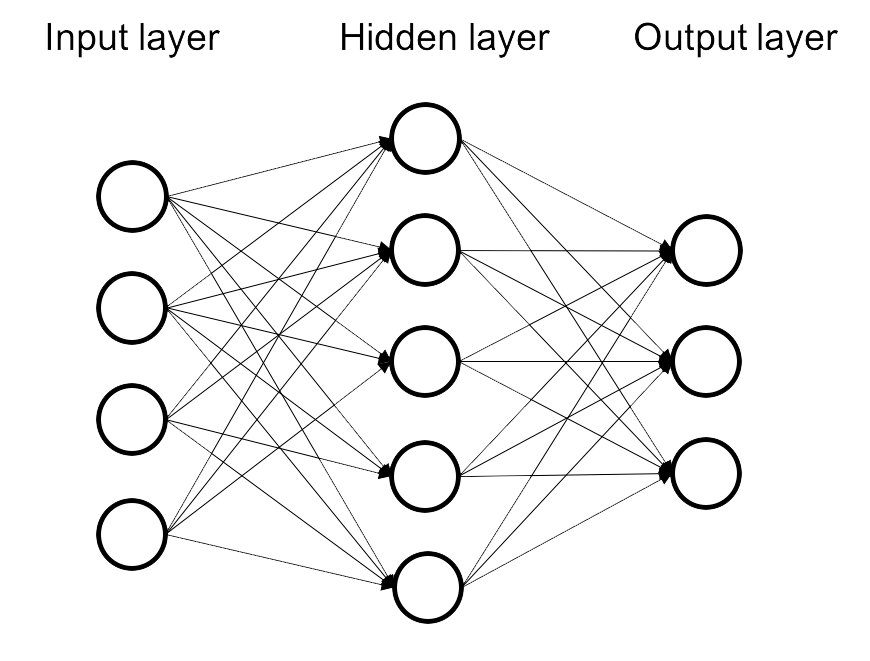
\includegraphics[width=0.45\linewidth]{shallow}
			\subcaption{Shallow architecture}
		\end{subfigure}
		\vskip\baselineskip
		% Start with figure tfrecord
		\begin{subfigure}[b]{\textwidth}
			\centering
			\captionsetup{justification=centering}
			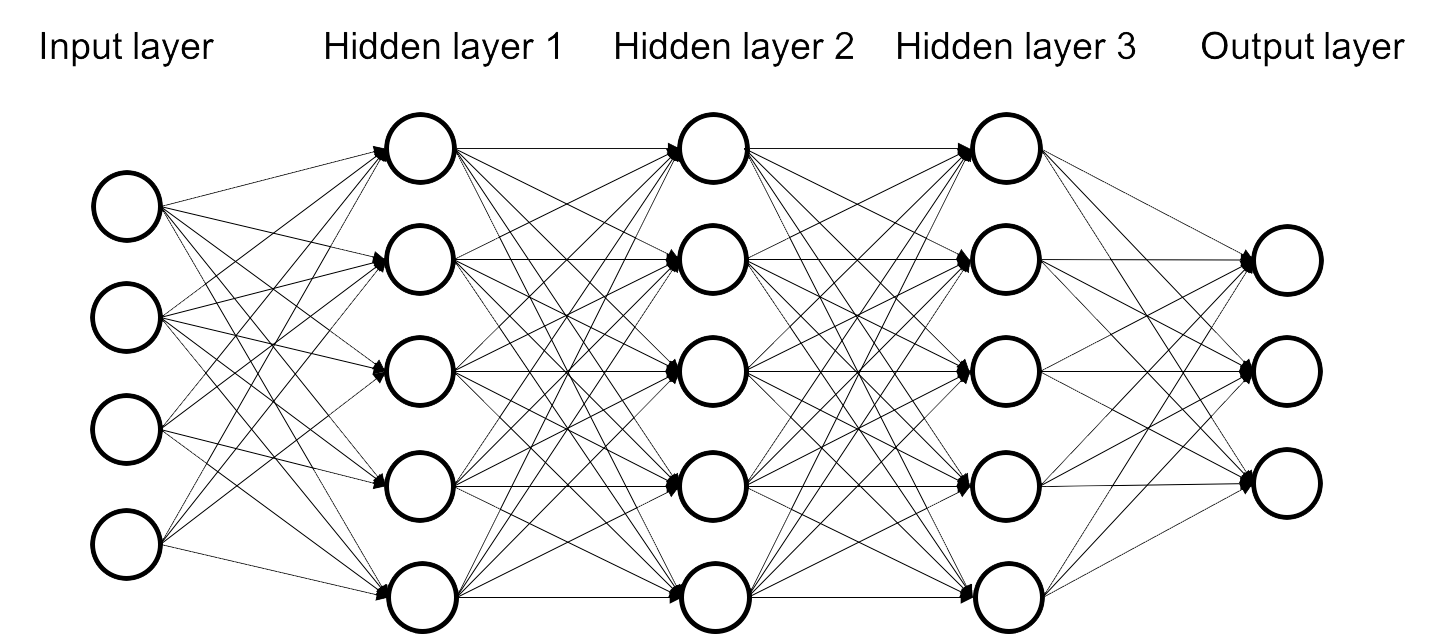
\includegraphics[width=0.6\linewidth]{dnn}
			\subcaption{Deep architecture}
		\end{subfigure}
		
		\caption{Comparison between shallow networks and deep neural networks \cite{Di2018}}
		\label{fig:mesh48}
	\end{figure} 

	% !TeX spellcheck = en_GB
% CNN explanation

\label{section:cnn}

	One of the most explored implementations is the one related to \acrfull{cnn}. This maintain the basic idea of receiving some inputs and apply a dot product operation to them before subject the data to a non-linear function but with the difference that input data are expected to be images \cite{Karpathy2016}. The architecture of a \acrlong{convnet} is based on the organization of the Visual Cortex in the human brain. This means that single neurons responds to some stimuli only in a certain region of the visual field, the Receptive Field. Then, a collection of these fields overlap with each other so as to cover the full visual space \cite{Saha2018}.
	
	About the input data, it is introduced as a matrix instead of as a row vector. Then, the architecture of the layers adapt to the fact that input data are images. They do not consist of a single row of neurons, but they have a shape constituted by three dimensions: heigh, width and depth \cite{Karpathy2016} \todo{include image?}. In this way, the net can capture the spatial and temporal relations present in an image by applying some filter functions. With this construction, the model can be trained with a smaller number of parameters and also reuse the weights.
	
	A \acrlong{convnet} can be described as a sequence of layers in which every layer converts a volume of activation results from the previous layer to another by computing a differentiable function. The architecture of a \acrshort{cnn} is always composed by three type of distinguishable layers which are \textit{Convolutional}, \textit{Pooling} and \textit{\acrlong{fc}}. A normal architecture will follow the next succession of layers \cite{Karpathy2016}:
	
	\begin{itemize}
		\item INPUT: this represents the image at the entrance of the whole model. It commonly is a 3\acrshort{d} matrix , one dimension per channel of colour, and contains the values of the original pixels.
		\item CONVOLUTIONAL: considering the neurons that are connected to a region of the input image, this layer computes their output by performing a dot product between the weights and the value of the pixels. The depth of the resulting data will coincide with the number of filters used.
		\item POOL: this performs a fixed operation that consists of a downsampling of the spatial dimension. It typically reduces by half the height and the width of the input image.
		\item \acrshort{fc}: this is the final layer which gives the output of the whole net. It is a vector-shape layer and is completely connected to the previous layer. In a classification task the number of neurons matches the amount of classes of the problem.
	\end{itemize}
	
	Note that this list represents the order of the layers in the architecture, however, the number of layers of each type vary depending on how the model is designed and how deep it is desired to be. For example, some examples of deep architectures can be found later in section \ref{subsection:vgg}, in table \ref{table:3}.
	
	With this building, a \acrlong{convnet} passes the information of the pixels layer by layer while reducing the input images in a way that is much easier to process. This is performed without missing any feature since all of them are essential to compute a good prediction outcome.
	
	In the convolutional layer, a convolution operation is performed for each small region of the input image. The element that carries out this operation is called \textit{kernel} or \textit{filter}. This partial region that the kernel covers in the input data is set by deciding the height and the width as a designing parameter. About the depth, it must match the depth of the input data so the filter can slide trough the image along its 2\acrshort{d} and obtaining the results of the convolution operation by computing between the pixels inside the region and the values of the filter. An example can be observed in figure \ref{fig:mesh11}. For each filter, a 2\acrshort{d} activation map is obtained after subjected the result of the convolution to a non-linear operation as the \acrfull{relu} function. Finally, we will pack all these in a unique volume that will consists in the output of the convolutional layer \cite{Karpathy2016}. For example, if we have a number of 64 filters, we will get then a group of 64 2\acrshort{d} activation maps that will be the input of the next layer. Traditionally, it was the first convolutional layer the one that was responsible of capturing low-level features related to edges or colours in the image. The upper layers were the ones in charge of extracting high-level features so the network was able to understand the image similar to how the humans do \cite{Saha2018}.
	
	\begin{figure}[ht]
		\centering
		\captionsetup{justification=centering}
		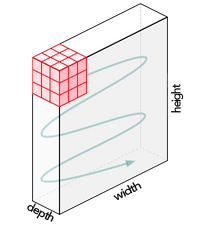
\includegraphics[scale=0.6]{movement-of-kernel}
		\caption{Movement of the kernel represented as a red block along the width and the height of the original input image. It is clear that it occupies the whole depth of the input image. The arrow indicates an approximation of the movement that the filter follows \cite{Saha2018}.}
		\label{fig:mesh11}
	\end{figure}

	We have included how the input interacts with the convolutional layer and also introduced the concept of depth of the resulting volume. However, it is needed to explain the how the total size of this output is computed and what it depends on. There are three main parameters that play a role in this decision: \textit{depth}, \textit{stride} and the \textit{zero-padding} \cite{Karpathy2016}.
	
	\begin{itemize}
		\item DEPTH: it is a hyperparameter that corresponds to the amount of kernels used in the convolutional layer when learning from the input.  The set of neurons that extent through the depth dimension operating in the same region is called depth column. This is the previous mentioned red block shown in figure \ref{fig:mesh11}.
		\item STRIDE: this indicates the displacement of the sliding filter along the image. If it has a value of 1 (non-strided), this means that the kernel will shift a position of one pixel along the width. When it is set to 2, then it moves two pixels. It rarely has values greater than 2. The moving process consists on the filter going from right to left with a hop determined by the stride value. When the right margin is reached, then it jumps to the beginning of the next row from the left margin and repeats the process in the same way until the image is completed \cite{Saha2018}. The bigger the stride, the smaller the size of the output volume.
		\item ZERO-PADDING: this is also called just \textit{padding}. It consists on adding zeros to the borders of the image. What is a hyperparameter in design is the size of this padding. This allows to control the width and height of the output volume so we can keep it the same through the different layers. When it is indicate a "valid padding", it means that no padding is added and the output size will be reduced. If we indicate "same padding", then it has a value of 1 and means that the resulting volume will have the size of the input \cite{Keras}.
	\end{itemize}

	As shown below, the total size of the obtained volume, $D$, can be computed as function of the input size, $W$, the spatial 2\acrshort{d} dimensions of the convolutional filter, $F$, the stride of the filters shifting, $S$,  and the amount of padding in the zero-padding, $P$ \cite{Karpathy2016}. 
	
	\[ D = \frac{W - F + 2P}{S} + 1 \]
	
	The convolutional layers can be grouped all together, one after another, but they are usually interpolated by what it has been previously defined as \textit{pooling} layer. This habit has the objective of reducing the the width and the height of the resulting volumes in a progressive manner in order to decrease the total number of training parameters and control the computational cost, and, therefore to avoid overfitting \cite{Karpathy2016} \todo{Include definition of overfitting or just cite it}. There can be performed two types of pooling operation: the max-pooling or the average-pooling. The former just returns the maximum value from the portion of the image where the filter is placed. The latter, computes the average of all the values in this portion \cite{Saha2018}. The pooling layer acts in an independent way on every input depth level. 
	
	Two hyperparameters are needed in order to configure the spatial portion in which the pooling is computed: the  filter size, related to length of height and width, and the stride. However, for this operation zero parameters are introduce since it consists on a fixed operation over the input data. In figure \ref{fig:mesh12}, it is shown how the max-pooling operation is performed \cite{Karpathy2016}. 
	
	\begin{figure}[ht]
		\centering
		\captionsetup{justification=centering}
		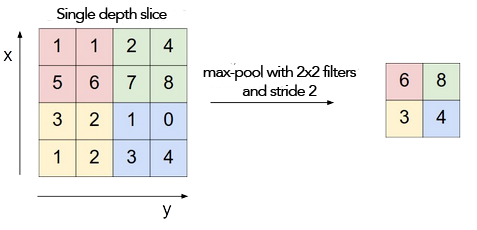
\includegraphics[scale=0.7]{max-pooling}
		\caption{Max-pooling operation with a filter size of 2 and a stride of 2 for a single depth filter. Each colour represents a the action portion for each operation \cite{Karpathy2016}}
		\label{fig:mesh12}
	\end{figure}
	
	Together a convolutional layer and a pooling layer constitute a complete layer structure typical in a \acrlong{convnet}. The number of these complete layers can vary depending on the design and the task needs. These represent the main core of the network before passing to the last layers and calculating the final output \cite{Saha2018}.
	
	For the final step, a common way of acting is to apply some non-linear activations in order to learn from the high-level features resulted from the output volume of the last convolutional layer. This takes place in the \acrlong{fc} layers ending the model. This part has the shape of a Fully-Connected layer, as the one described in the basic model of \acrshort{ann}. To make the weights from the convolutional layers available to feed this last part of the model, it is necessary to flatten the output volume and obtain a column vector. The learning process is possible due to a backpropagation operation performed in every epoch of training. As a total output, the values that represent the classification of the different samples into one or another category are obtained \cite{Saha2018}. A common classification technique is the one called \textit{Softmax}. This normalizes the result of the previous \acrshort{fc} layer into a vector whose values follow a distribution that total sum results in 1. This type of output is called \textit{soft predictions} and represent the probability for each sample of belonging to a category in the classification \cite{Mahmood2018}. However, there exists other activation functions that can compute the classification output in other ways. 
	
	In figure \ref{fig:mesh13} an scheme of a common \acrlong{cnn} is shown. This takes an input image, compute the features along three groups of convolutional layer plus max-pooling and, finally, includes three \acrlong{fc} layers, being the last one a softmax function layer with as many neurons as classes that gives the soft predictions for this image of belonging to each class.
	
	\begin{figure}[ht]
		\centering
		\captionsetup{justification=centering}
		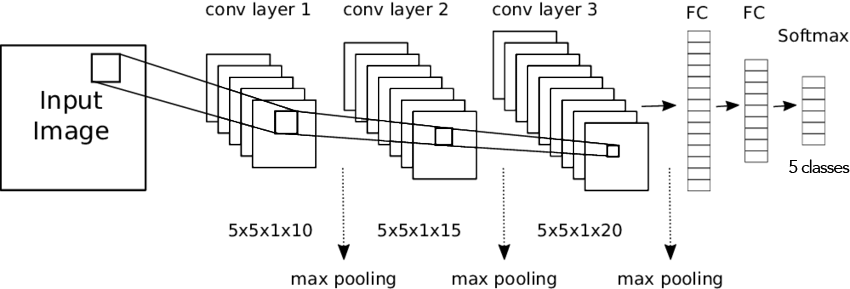
\includegraphics[scale=0.4]{cnn}
		\caption{Representation of a typical CNN model \cite{Hinz2016}}
		\label{fig:mesh13}
	\end{figure}

	\acrfull{cnn} were originally designed to work with images but they have been applied to other fields as audio. An image can be defined as a matrix of values, i.e. pixels, in two or three dimensions, so the only prerequisite to use a \acrshort{cnn} is to have the input data in this form. For audio researching, it has been commonly used the log-scaled mel spectrogram, that is a way of representing audio in a scale different than frequency that is more similar to humans perception. It has been used in plenty of works with \acrshort{cnn} and also combined with other techniques \cite{Salamon2017} \cite{Piczak2015} \cite{Kumar2017}.
	
	
	

	

	
	
	
	
	


\subsection{\acrfull{vgg} model}
\label{subsection:vgg}

	\acrshort{cnn} are usually able to achieve really good results and even improve human skills on \acrlong{cv} tasks, for example, on recognizing object in an image. With the exponential growth of the researching works on this field, some challenges have appeared so as to promote the creation of new systems and test their efficiency and results. This is the case of the \acrfull{ilsvrc}, based on the database of the same name, ImageNet. As a solution for the proposed exercise, the investigators from the \acrfull{vgg} in the University of Oxford implemented a new system achieving the first position and winning the challenge in 2014 \cite{ImageNet2014}. The work they proposed consists of a study of the depth in a \acrlong{convnet} architecture and how this can affect to the accuracy on the goal of large-scale image recognition \cite{Simonyan2015}. To try this, it was necessary to increase the number of layers in the network, which was viable due to use a small size of convolutional filters in all of them.

	For the training step of their system, they used an input image with standard size of $224 \times 224$ in \acrshort{rgb} format. The principles to build the architecture are detailed below:
	
	\begin{itemize}
		\item The input image crosses a bunch of convolutional layers in which the kernel has a size of $3 \times 3$.
		\item The convolutional stride has a value of 1 pixel.
		\item The padding is fixed to 1 pixel, so the dimensions of the input do not change during the convolution.
		\item Max-pooling is also included with a window size of $2 \times 2$ and a stride value of 2 pixels.
		\item Two \acrfull{fc} layers with 4096 channels after all the \acrlong{convnet} layers.
		\item One \acrshort{fc} layer with 1000 channels to perform the \acrshort{ilsvrc} classification.
		\item A soft-max layer is employed for the final layer.
		\item All hidden \acrlong{convnet} layers use the non-linear function \acrshort{relu} as activation function.
	\end{itemize}
	
	All the designs that the creators came up with are based on these initial guidelines, except from just one case where \acrfull{lrn} is applied, previously mentioned in subsection \ref{subsection:ann-cnn}. They just differ from each other on the number of layers, starting with 11 the first approach and ending with 19 the last one. The different architectures are specified in the table \ref{table:3} \cite{Simonyan2015} and are ordered from A to E.
	
	% Table configuration of VGG
	\begin{table}[t!]
		\begin{center}
			\captionsetup{justification=centering}
			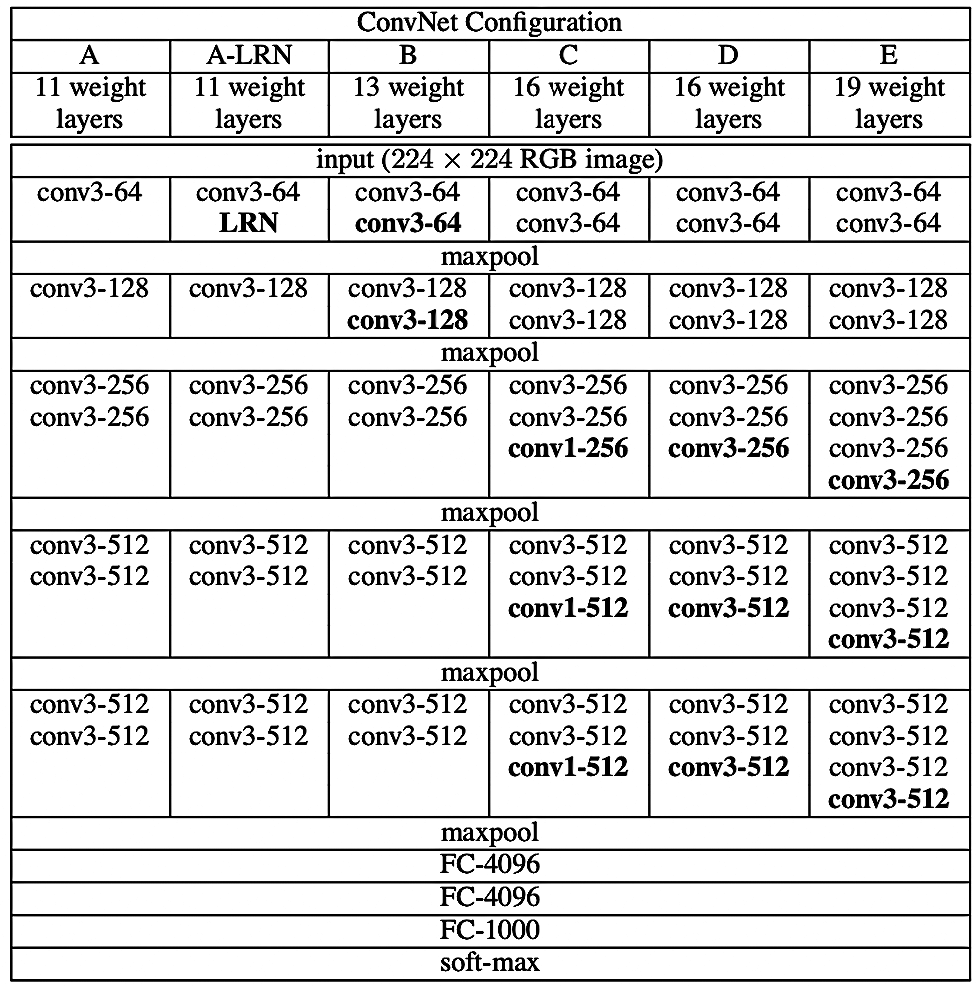
\includegraphics[scale=0.4]{vgg-confs}
			\caption{VGG ConvNet configurations.}
			\label{table:3}
		\end{center}
	\end{table}

\subsection{\acrshort{vgg}ish model}
\label{subsection:vggish}

	The model we used in our project for feature extraction presents a configuration with principles similar to the ones explained in the previous subsection \ref{subsection:vgg} but with slight changes that their developers have included in order to adapt it to the audio approach. As previously mentioned in subsection \ref{subsection:data-access}, the implementation of this model has been obtained from the website of the database Audio Set, in which a code repository is public available \cite{Ellis2017} and all the information about the implementation is included.
	
	The architecture is based in the configuration A from table \ref{table:3} with 11 weights. The differences respect to the original network are listed below: 
	\begin{itemize}
		\item The input size was changed from $224 \times 224$ to $96 \times 64$ because of the log-mel spectrogram audio inputs.
		\item They built the implementation with just four groups of convolutional and max-pool layers, instead of five.
		\item For the last \acrshort{fc} layer, they decided to build it just with 128 channels since it is the layer that compacts the final embedding and defines its dimensions.
		\item Also the final \textit{Softmax} layer is not used.
	\end{itemize}
	Figure \ref{fig:mesh2} shows how the configuration of the final \acrshort{vgg}ish model looks.
	
	\begin{figure}
		\centering
		\captionsetup{justification=centering}
		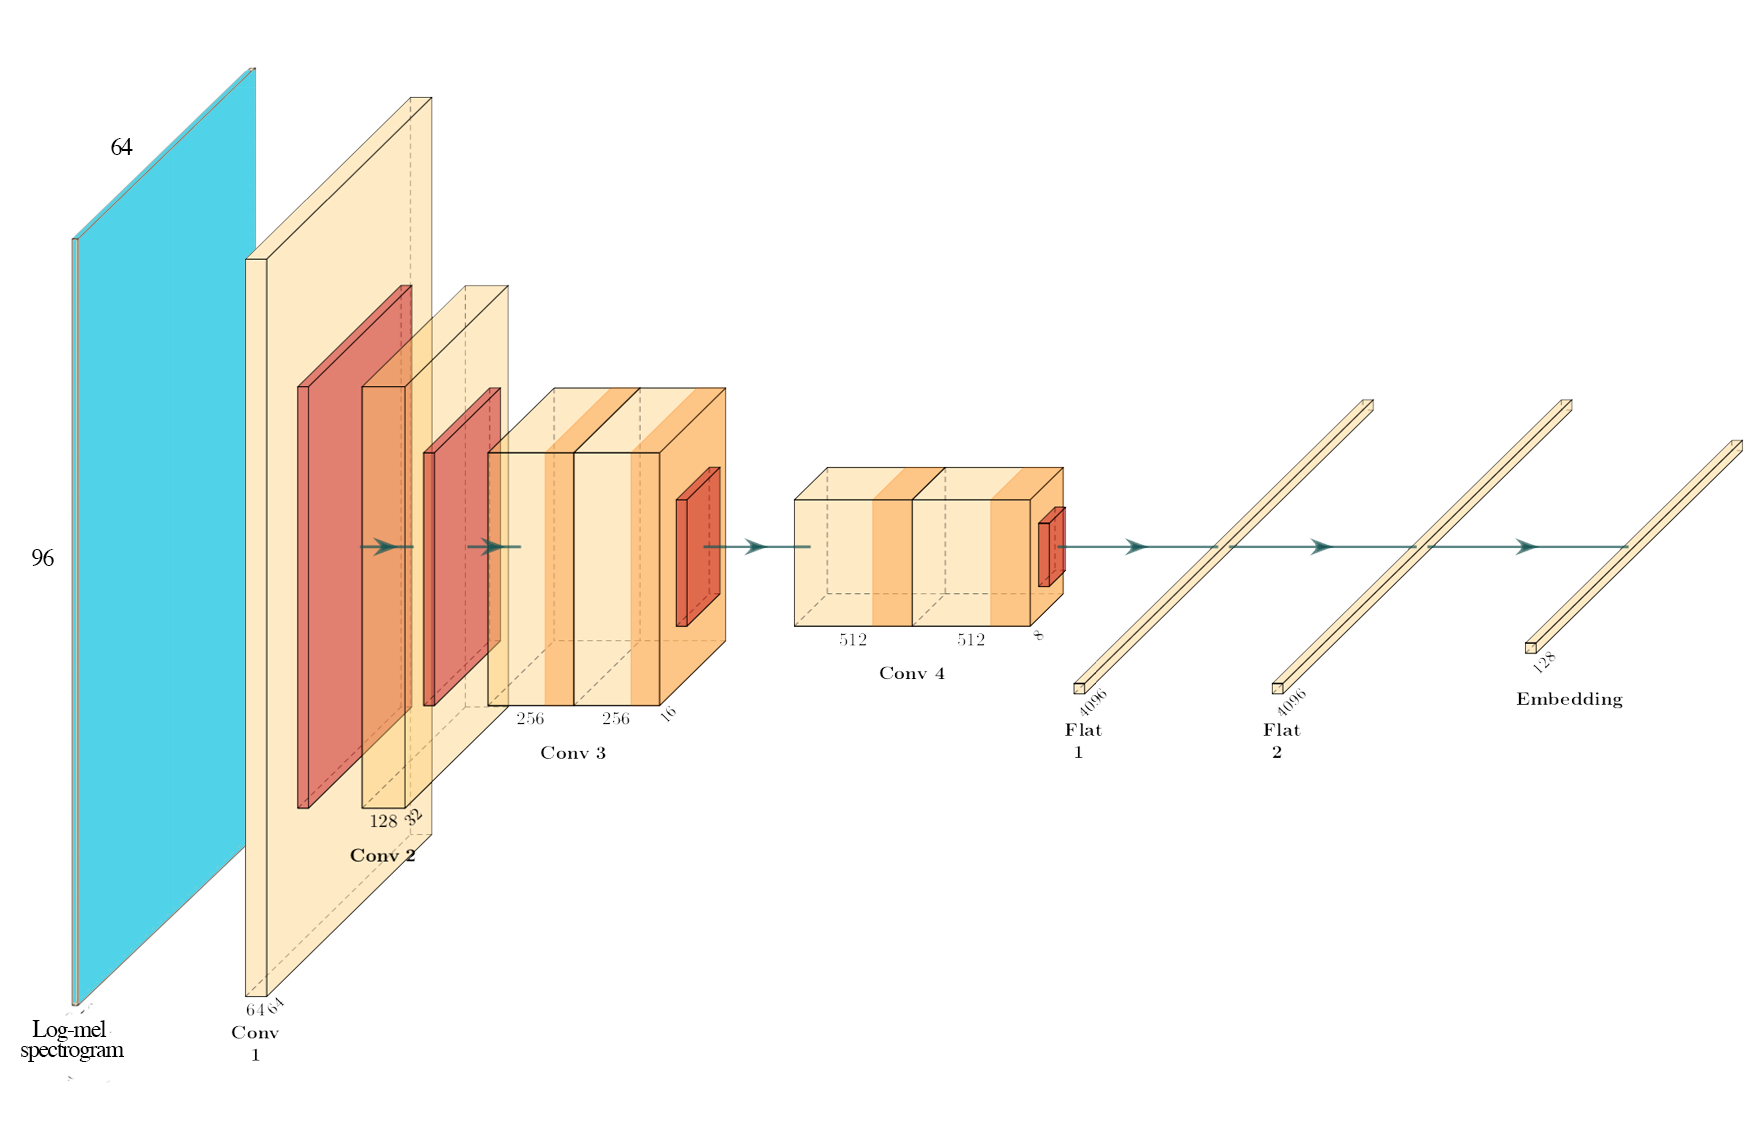
\includegraphics[scale=0.25]{model-vggish}
		\caption{VGGish architecture}
		\label{fig:mesh2}
	\end{figure}

\subsubsection*{Input stage}

	Before passing the data through the whole \acrshort{cnn}, a preprocessing stage has been included by the developers in which the input audio will suffer some transformations. 

	\begin{enumerate}
		\item In the first place, after loading the input audio, the sample rate and the number of channels are checked to be 16 kHz and monochannel, otherwise the file is transformed to satisfy these conditions.
		\item When the data is ready, the next step is computing the spectrogram. For this, it is necessary to calculate first the \acrfull{stft} of the signal. The operation is performed by using a sliding Hanning window of 25 ms with a hop size of 10 ms. As a result, just the magnitudes that correspond to the positive frequencies are retained, since the ones corresponding to the negative part of the spectrogram are redundant.
		\item  Transforming the spectrogram to Mel scale is what follows. To do so, they compute all mel frequency bins that are going to modify the values of the spectrogram in frequency domain by following a hertz to mel conversion formula, that can be found in appendix \ref{section:spectrogram-mel-scale}. The result is a mel spectrogram from 125 Hz to 7,500 Hz divided in 64 bins.
		\item Then, the log-mel spectrogram is calculated by doing the logarithm of the previous result plus a small offset value to avoid the logarithm of $0$.
		\item As a final step, they compute a framing operation over the log-mel spectrogram. The resulting are non-overlapping examples of 0.96 seconds, in which 64 mel bands and 96 frames are contained, each frame with a duration of 10 ms.
	\end{enumerate}

	Therefore, the result obtained is an ensemble of 10 frames, approximately one per second, each of them with size $96 \times 64$, i.e, 96 frames and 64 mel bands.

\subsubsection*{Embedding stage}

	Once the initial processing part is done and the log-mel spectrogram matrix is computed and divided into the desired number of frames, it is used as input data for the \acrshort{vgg}ish \acrshort{cnn}. After all the computations inside the network, each example is converted into an embedding of size 128 giving a result of one of these per second of the original audio file.

\subsubsection*{Postprocessing stage}

	As final step, they performed some post-processing of the resulting embeddings. A \acrfull{pca} \cite{Abdi2010} transformation is done joint with a whitening process. Also, a quantization to 8 bit for each embedding element. All these actions are computed with the purpose of making the final output compatible with the embeddings obtained from the YouTube-8M database.

	\todo{Transfer learning and why choosing this type}
